\chapter{MAPA DOS RESULTADOS SUPLEMENTARES}
\label{ap:resultados}

Os relatórios HTML publicados contêm os rankings completos, curvas de perda, matrizes de vencedores $\Wmat$ e de inversões $\Rmat$, os quatro indicadores de preservação e metadados de execução, sob o esquema $\Wmat/\Rmat$ vigente (Capítulo~4). Este apêndice registra os artefatos utilizados na auditoria do relatório, incluindo a resolução da limitação de disponibilidade de dados descrita na Seção~\ref{sec:resultados-guia} e detalhada no Apêndice~B. A página inicial da publicação é:

\begin{center}
\url{https://paulorenatoaz.github.io/coinfosim/}
\end{center}

\section{Cenários principais}
\label{ap:resultados-cenarios}

\begin{longtable}{p{2.5cm}p{1.5cm}p{9.2cm}}
\caption{Relatórios de cenário auditados}\label{tab:appendix-scenarios}\\
\toprule
\textbf{Dataset} & \textbf{ID} & \textbf{Relatório} \\
\midrule
\endfirsthead
\toprule
\textbf{Dataset} & \textbf{ID} & \textbf{Relatório} \\
\midrule
\endhead
Occupancy Detection & 000002 & \url{https://paulorenatoaz.github.io/coinfosim/reports/scenarios/000002_occupancy_baseline_full/occupancy_baseline_scenario_report_full_000002.html} \\
\addlinespace
UCI Air Quality & 000005 & \url{https://paulorenatoaz.github.io/coinfosim/reports/scenarios/000005_air_quality_baseline_full/air_quality_scenario_report_full_000005.html} \\
\addlinespace
SUPPORT2, classificadores originais & 000007 & \url{https://paulorenatoaz.github.io/coinfosim/reports/scenarios/000007_support2_baseline_full/support2_scenario_report_full_000007.html} \\
\addlinespace
SUPPORT2, Random Forest & 000008 & \url{https://paulorenatoaz.github.io/coinfosim/reports/scenarios/000008_support2_baseline_full/support2_scenario_report_full_000008.html} \\
\bottomrule
\sourcebelow{elaboração própria com base nos relatórios publicados do \CoInfoSim}
\end{longtable}

\section{Relatórios detalhados de Occupancy}

O cenário 000002 referencia os seguintes artefatos:

\begin{itemize}
  \item relatório do dataset: \url{https://paulorenatoaz.github.io/coinfosim/reports/scenarios/000002_occupancy_baseline_full/occupancy_dataset_report_full_000002.html};
  \item Real $\rightarrow$ Real, simulação 000006: \url{https://paulorenatoaz.github.io/coinfosim/reports/simulations/000006_occupancy_real_data_full/occupancy_real_data_monte_carlo_report_full_000006.html};
  \item Gaussiana única $\rightarrow$ Real, simulação 000007: \url{https://paulorenatoaz.github.io/coinfosim/reports/simulations/000007_occupancy_single_gaussian_to_real_full/occupancy_single_gaussian_to_real_monte_carlo_report_full_000007.html};
  \item GMM $\rightarrow$ Real, simulação 000008: \url{https://paulorenatoaz.github.io/coinfosim/reports/simulations/000008_occupancy_gmm_to_real_full/occupancy_gmm_to_real_monte_carlo_report_full_000008.html}.
\end{itemize}

\section{Relatórios detalhados de Air Quality}

O cenário 000005 é a entrada principal e referencia:

\begin{itemize}
  \item relatório do dataset: \url{https://paulorenatoaz.github.io/coinfosim/reports/scenarios/000005_air_quality_baseline_full/air_quality_dataset_report_full_000005.html};
  \item Real $\rightarrow$ Real, simulação 000015: \url{https://paulorenatoaz.github.io/coinfosim/reports/simulations/000015_air_quality_real_data_full/air_quality_real_data_monte_carlo_report_full_000015.html};
  \item Gaussiana única $\rightarrow$ Real, simulação 000016: \url{https://paulorenatoaz.github.io/coinfosim/reports/simulations/000016_air_quality_single_gaussian_to_real_full/air_quality_single_gaussian_to_real_monte_carlo_report_full_000016.html};
  \item GMM $\rightarrow$ Real, simulação 000017: \url{https://paulorenatoaz.github.io/coinfosim/reports/simulations/000017_air_quality_gmm_to_real_full/air_quality_gmm_to_real_monte_carlo_report_full_000017.html}.
\end{itemize}

Os valores de $\rankrho$, $\AW$, $\AR$, $\DR$ e $\SR$ do PDF foram computados diretamente pelo código atual a partir dos resultados brutos por replicação regenerados deste cenário, e conferidos contra o payload \texttt{predictive\_cooperation\_profile} embutido no \texttt{scenario.json} republicado, além das visualizações bidimensionais de dados reais, Gaussiana única e GMM. Esses valores são reportados no Capítulo~5 (Tabela~\ref{tab:air-final}), nos termos da Seção~\ref{sec:resultados-guia}.

\subsection{Extensão full-scale (cenário 000006)}

Conforme a política editorial do Capítulo~3 (Seção de proveniência), o cenário 000006 --- Air Quality em modo \textit{full-scale}, grade estendida até 1.024 amostras por classe --- é tratado como extensão suplementar e não é combinado com os valores do cenário 000005 no mesmo indicador. Seus artefatos são:

\begin{itemize}
  \item relatório do dataset: \url{https://paulorenatoaz.github.io/coinfosim/reports/scenarios/000006_air_quality_baseline_full-scale/air_quality_dataset_report_full-scale_000006.html};
  \item relatório do cenário: \url{https://paulorenatoaz.github.io/coinfosim/reports/scenarios/000006_air_quality_baseline_full-scale/air_quality_scenario_report_full-scale_000006.html};
  \item Real $\rightarrow$ Real, simulação 000018: \url{https://paulorenatoaz.github.io/coinfosim/reports/simulations/000018_air_quality_real_data_full-scale/air_quality_real_data_monte_carlo_report_full-scale_000018.html};
  \item Gaussiana única $\rightarrow$ Real, simulação 000019: \url{https://paulorenatoaz.github.io/coinfosim/reports/simulations/000019_air_quality_single_gaussian_to_real_full-scale/air_quality_single_gaussian_to_real_monte_carlo_report_full-scale_000019.html};
  \item GMM $\rightarrow$ Real, simulação 000020: \url{https://paulorenatoaz.github.io/coinfosim/reports/simulations/000020_air_quality_gmm_to_real_full-scale/air_quality_gmm_to_real_monte_carlo_report_full-scale_000020.html}.
\end{itemize}

Seus resultados brutos por replicação estão disponíveis para auditoria e regeneração nos mesmos termos dos demais cenários acadêmicos, mas não são tabulados no corpo do relatório por usarem um prefixo amostral não comparável a $n\leq512$.

\section{Relatórios detalhados de SUPPORT2}

O cenário 000007 contém SVM linear, regressão logística e Gaussian Naive Bayes; o cenário 000008 contém o experimento adicional de Random Forest. Ambos referenciam:

\begin{itemize}
  \item relatório do dataset: \url{https://paulorenatoaz.github.io/coinfosim/reports/scenarios/000008_support2_baseline_full/support2_dataset_report_full_000008.html};
  \item cenário 000007 --- Real $\rightarrow$ Real, simulação 000021: \url{https://paulorenatoaz.github.io/coinfosim/reports/simulations/000021_support2_real_data_full/support2_real_data_monte_carlo_report_full_000021.html};
  \item cenário 000007 --- Gaussiana única $\rightarrow$ Real, simulação 000022: \url{https://paulorenatoaz.github.io/coinfosim/reports/simulations/000022_support2_single_gaussian_to_real_full/support2_single_gaussian_to_real_monte_carlo_report_full_000022.html};
  \item cenário 000007 --- GMM $\rightarrow$ Real, simulação 000023: \url{https://paulorenatoaz.github.io/coinfosim/reports/simulations/000023_support2_gmm_to_real_full/support2_gmm_to_real_monte_carlo_report_full_000023.html};
  \item cenário 000008 --- Real $\rightarrow$ Real, simulação 000024: \url{https://paulorenatoaz.github.io/coinfosim/reports/simulations/000024_support2_real_data_full/support2_real_data_monte_carlo_report_full_000024.html};
  \item cenário 000008 --- Gaussiana única $\rightarrow$ Real, simulação 000025: \url{https://paulorenatoaz.github.io/coinfosim/reports/simulations/000025_support2_single_gaussian_to_real_full/support2_single_gaussian_to_real_monte_carlo_report_full_000025.html};
  \item cenário 000008 --- GMM $\rightarrow$ Real, simulação 000026: \url{https://paulorenatoaz.github.io/coinfosim/reports/simulations/000026_support2_gmm_to_real_full/support2_gmm_to_real_monte_carlo_report_full_000026.html}.
\end{itemize}

Os valores de $\rankrho$, $\AW$, $\AR$, $\DR$ e $\SR$ da Tabela~\ref{tab:support2-original} e da Seção~\ref{sec:support2-rf} foram computados diretamente pelo código atual: para o cenário 000007, a partir do payload \texttt{predictive\_\allowbreak cooperation\_\allowbreak profile} embutido no \texttt{scenario.json} republicado; para o cenário 000008, cujo \texttt{structural\_\allowbreak snapshot\_\allowbreak policy} é \texttt{regenerate\_\allowbreak from\_\allowbreak result\_\allowbreak data}, a partir dos resultados brutos por replicação das simulações 000024--000026 acima, usando

\begin{center}
\small\texttt{coinfosim.results.predictive\_profile.\allowbreak scenario\_predictive\_profile\_agreement}
\end{center}

\noindent diretamente (mesma função que o relatório HTML usa para renderizar o cenário sob demanda).

\section{Matrizes completas de projeções geométricas}
\label{ap:geometria-completa}

O corpo do relatório (Capítulo~4) mostra, para cada dataset, apenas a projeção bidimensional $(X_1,X_2)$ como comparação representativa entre dados reais, Gaussiana única e GMM. Esta seção reproduz a matriz completa de projeções par a par entre todos os canais, nos três braços, para os quatro cenários principais. Como no corpo do texto, essas figuras são inspeções exploratórias, não testes formais de aderência nem provas de preservação do perfil de cooperação preditiva (Seção~\ref{sec:provenance}).

\begin{figure}[H]
  \centering
  \caption{Matriz completa de projeções --- Occupancy Detection, dados reais}
  \label{fig:geom-occupancy-full-real}
  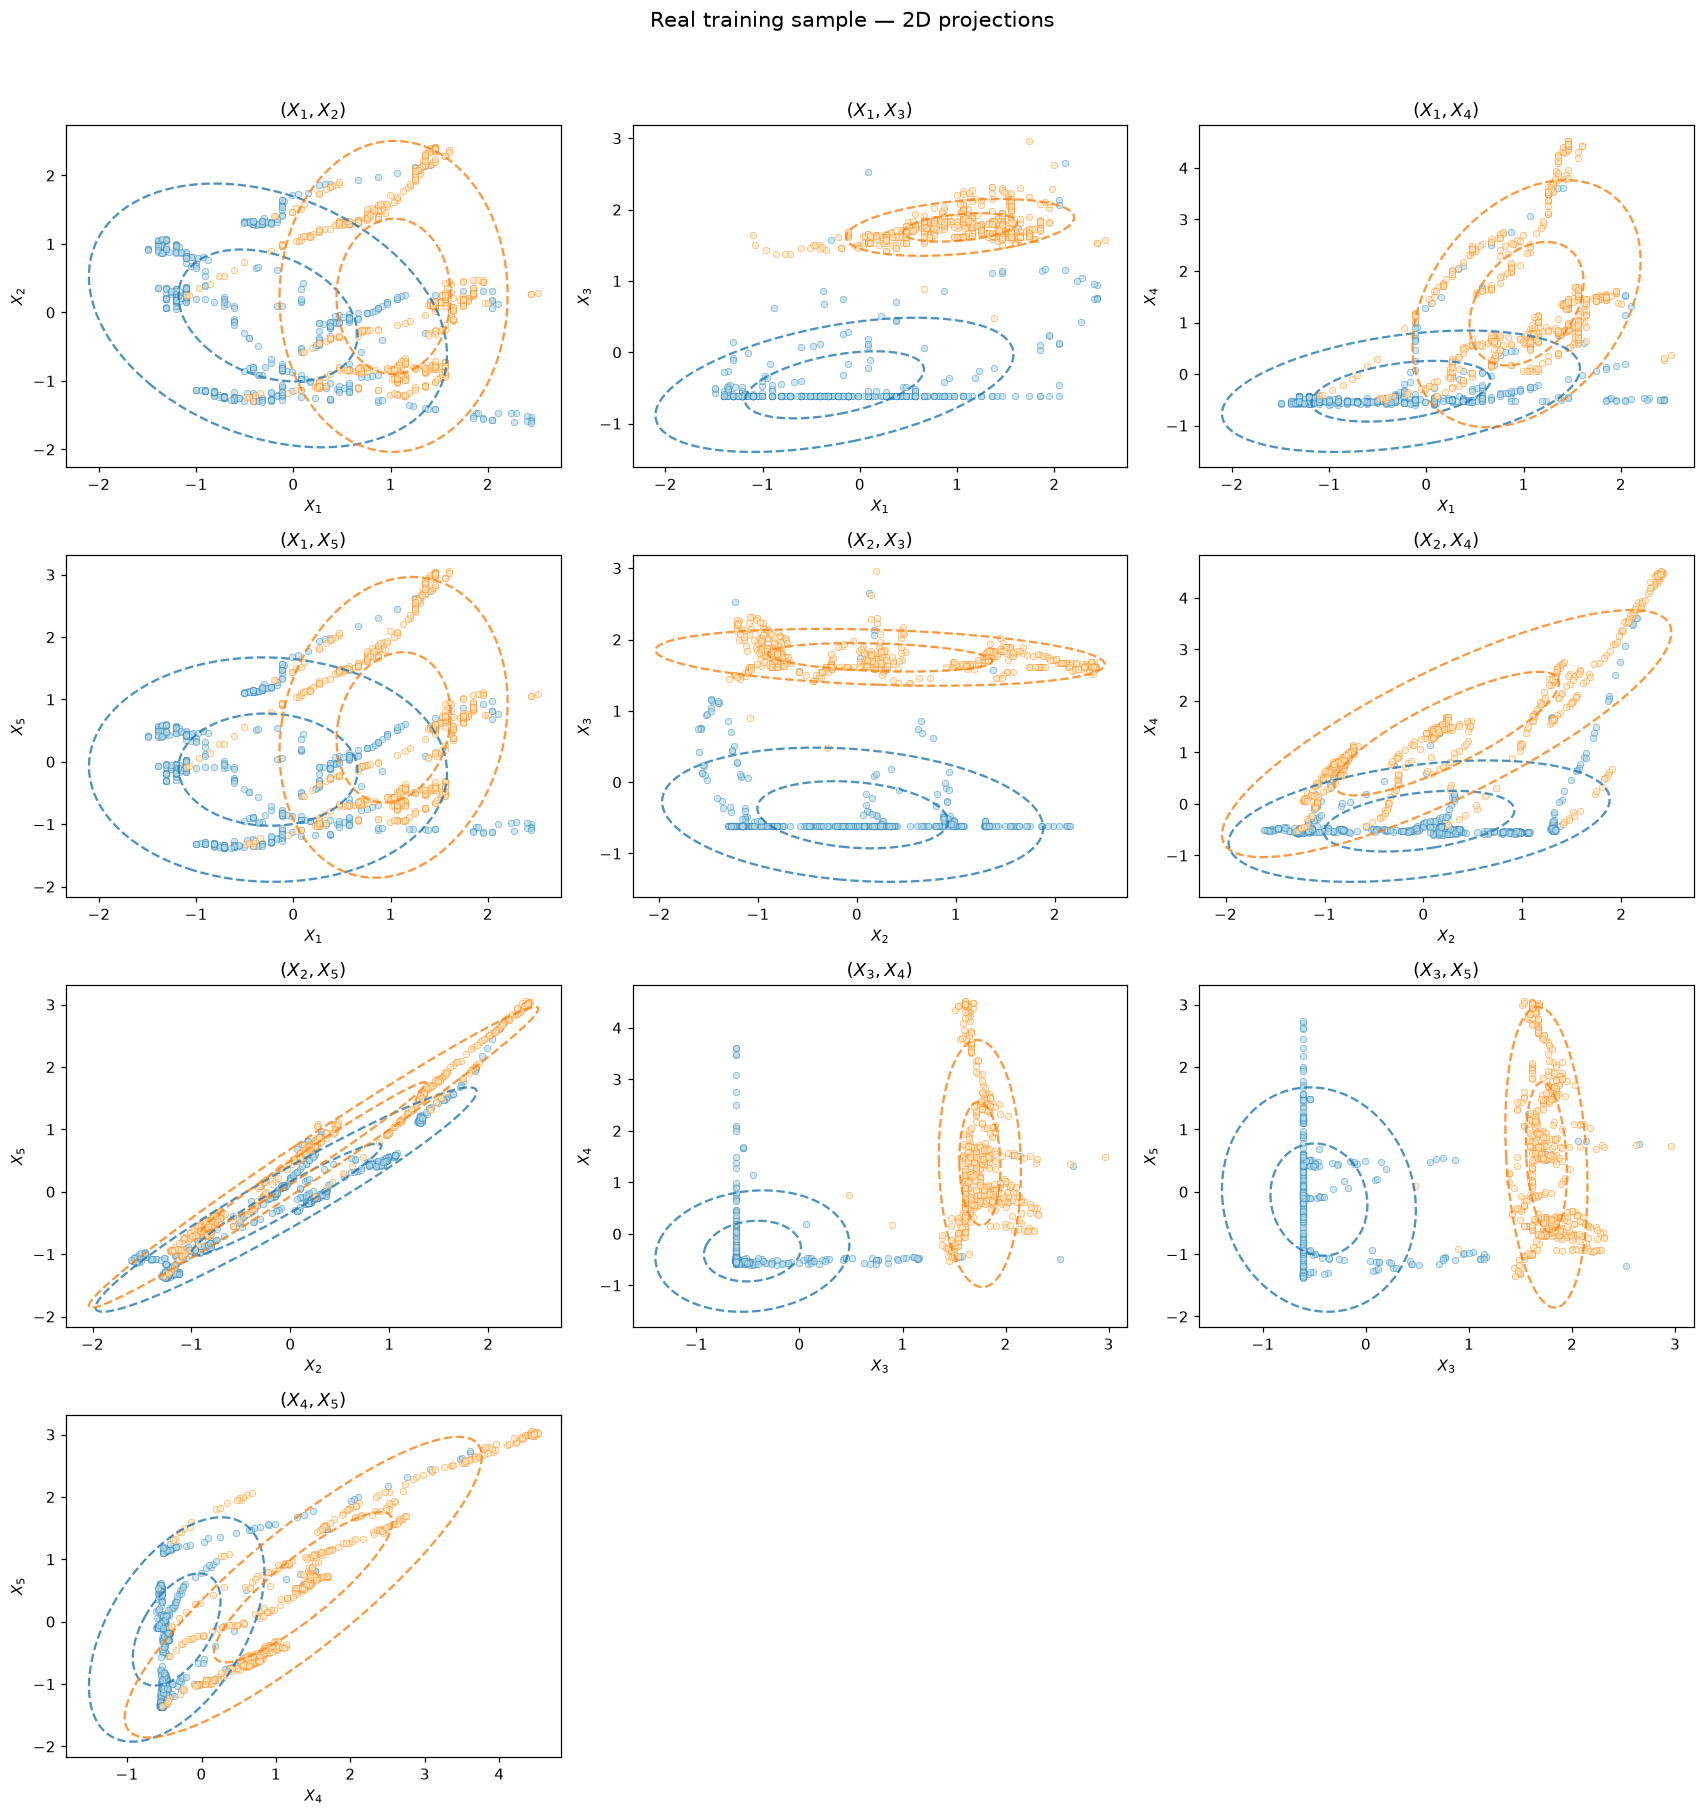
\includegraphics[width=\textwidth,height=0.85\textheight,keepaspectratio]{figures/geometry/occupancy/viz_2d_real_full_000002.png}
  \sourcebelow{relatório publicado do cenário Occupancy Detection 000002 do \CoInfoSim}
\end{figure}

\begin{figure}[H]
  \centering
  \caption{Matriz completa de projeções --- Occupancy Detection, Gaussiana única}
  \label{fig:geom-occupancy-full-gaussian}
  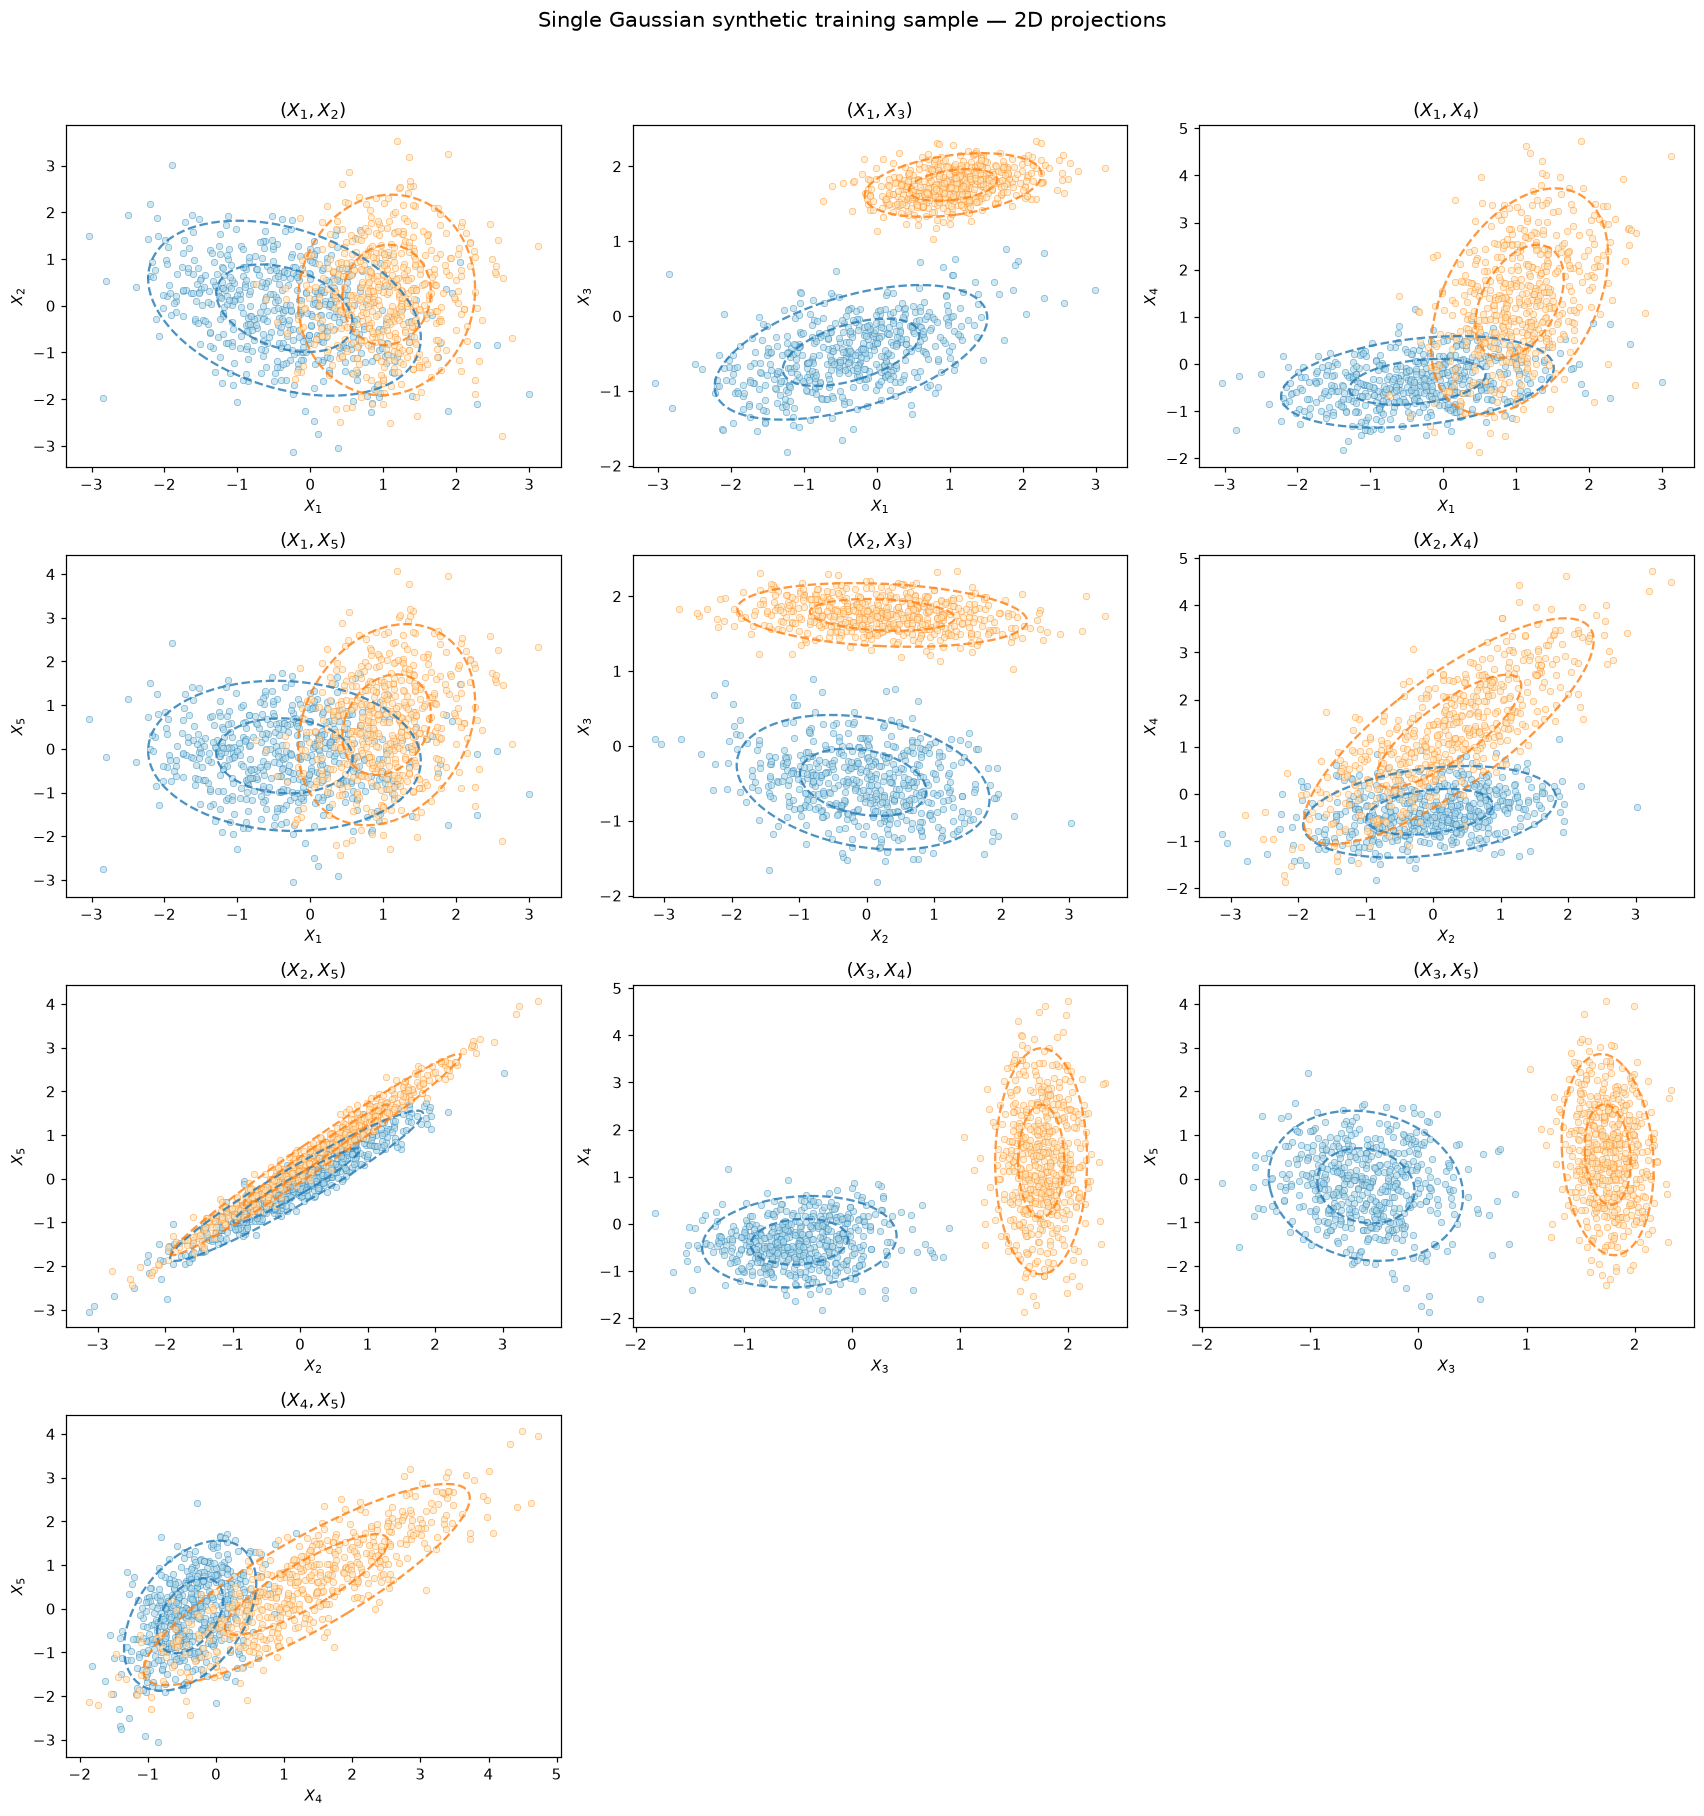
\includegraphics[width=\textwidth,height=0.85\textheight,keepaspectratio]{figures/geometry/occupancy/viz_2d_gaussian_full_000002.png}
  \sourcebelow{relatório publicado do cenário Occupancy Detection 000002 do \CoInfoSim}
\end{figure}

\begin{figure}[H]
  \centering
  \caption{Matriz completa de projeções --- Occupancy Detection, GMM}
  \label{fig:geom-occupancy-full-gmm}
  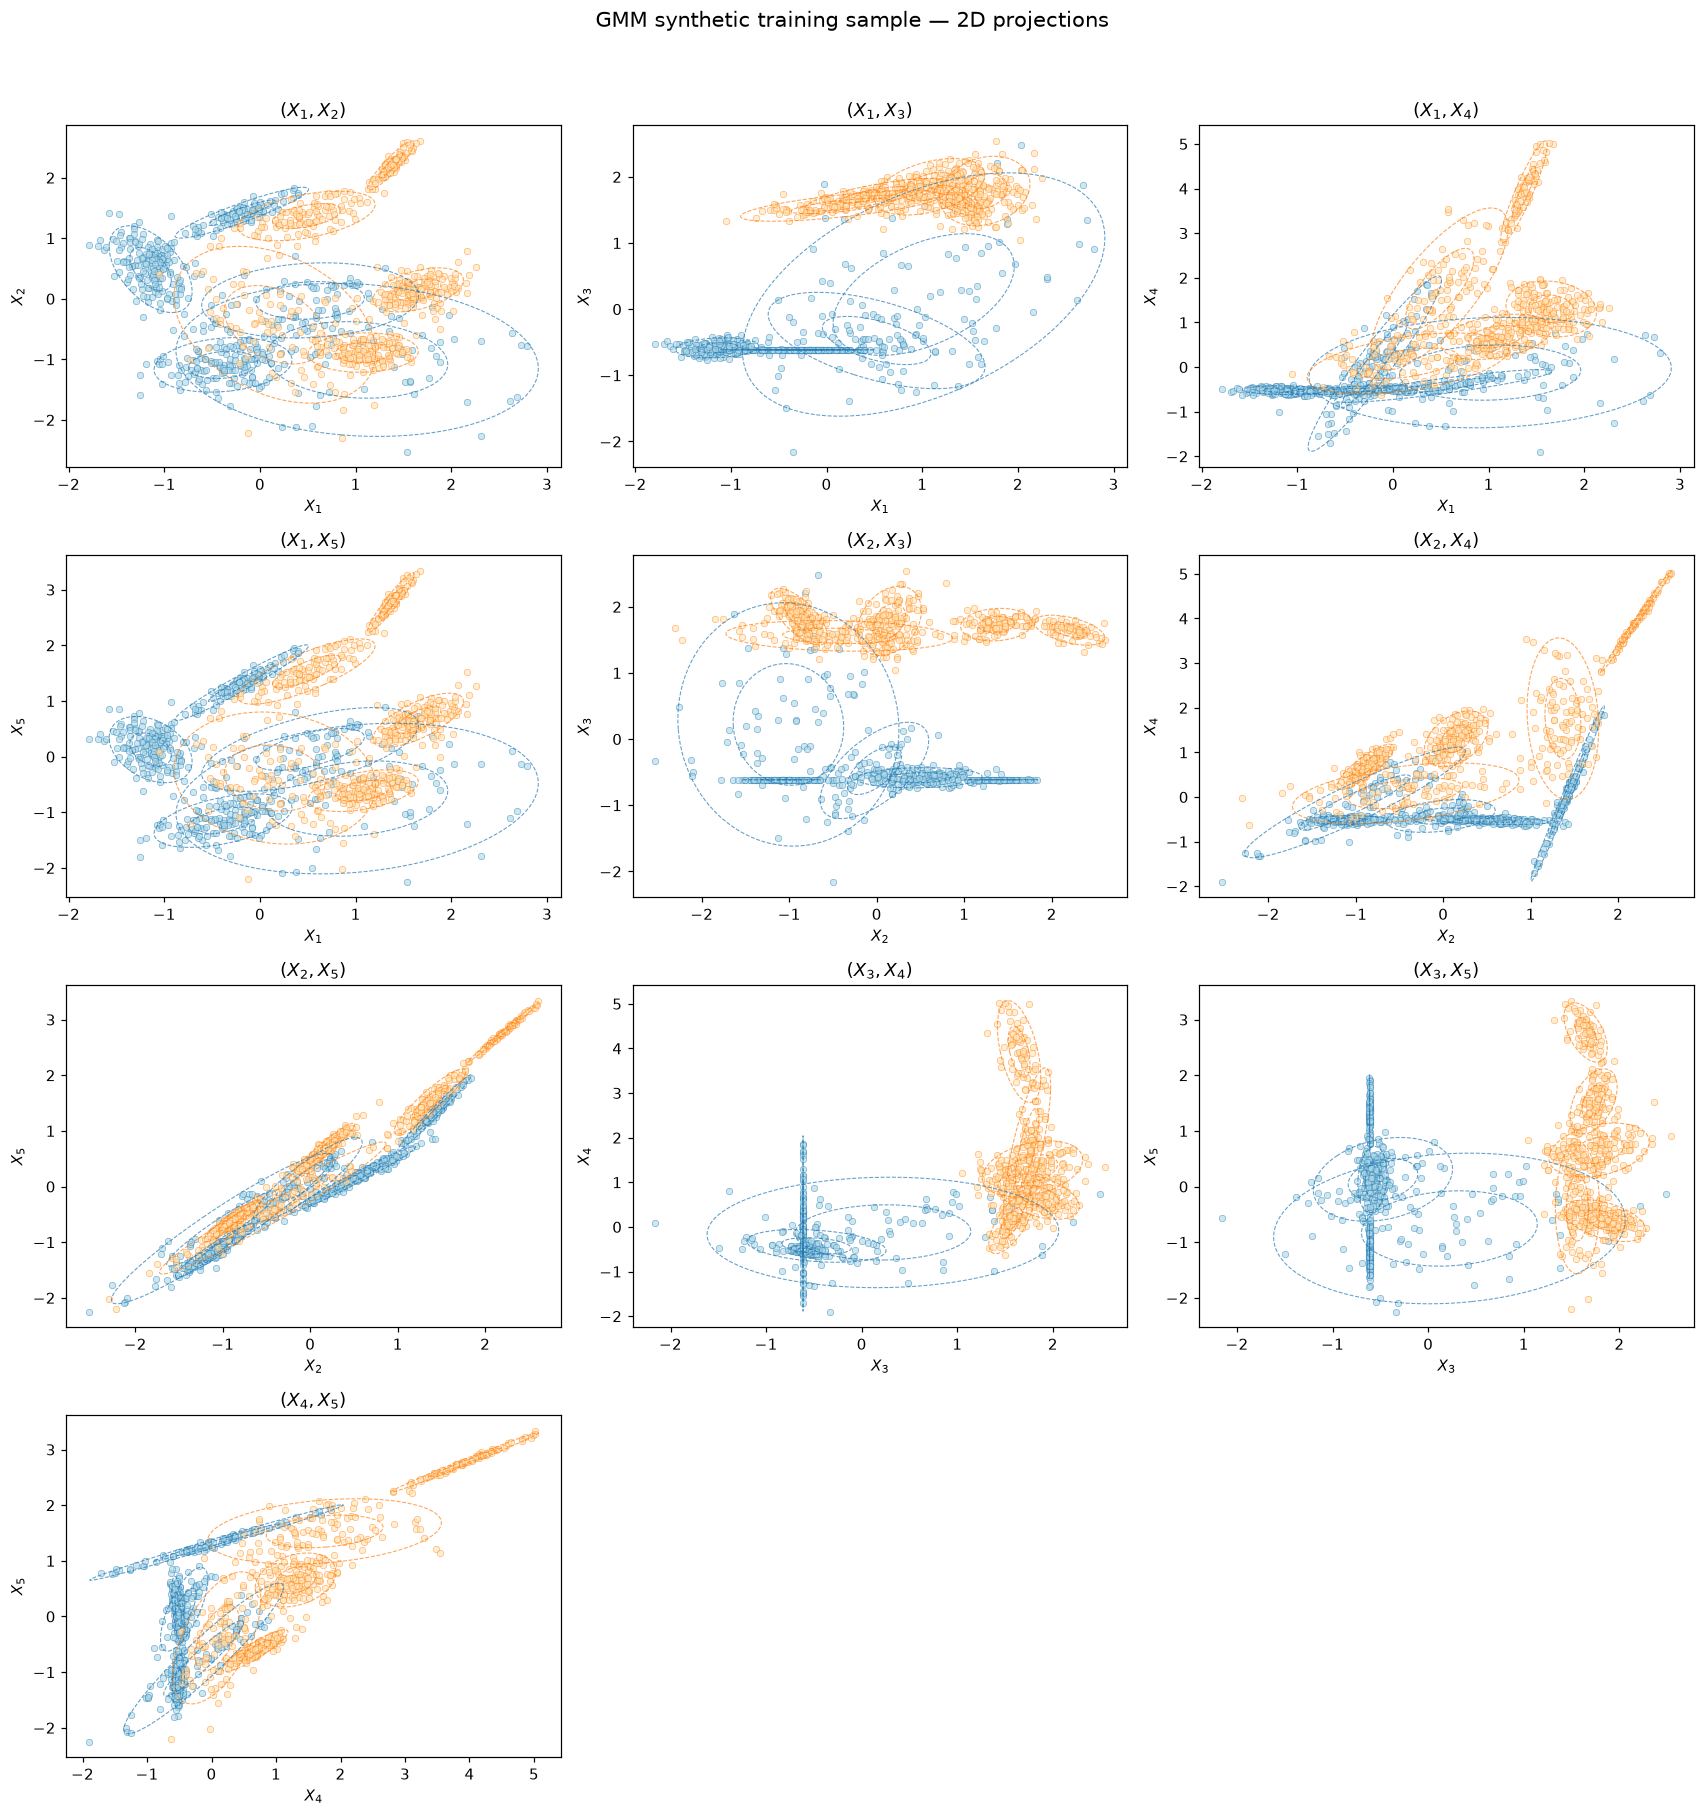
\includegraphics[width=\textwidth,height=0.85\textheight,keepaspectratio]{figures/geometry/occupancy/viz_2d_gmm_full_000002.png}
  \sourcebelow{relatório publicado do cenário Occupancy Detection 000002 do \CoInfoSim}
\end{figure}

\begin{figure}[H]
  \centering
  \caption{Matriz completa de projeções --- UCI Air Quality, dados reais}
  \label{fig:geom-air-full-real}
  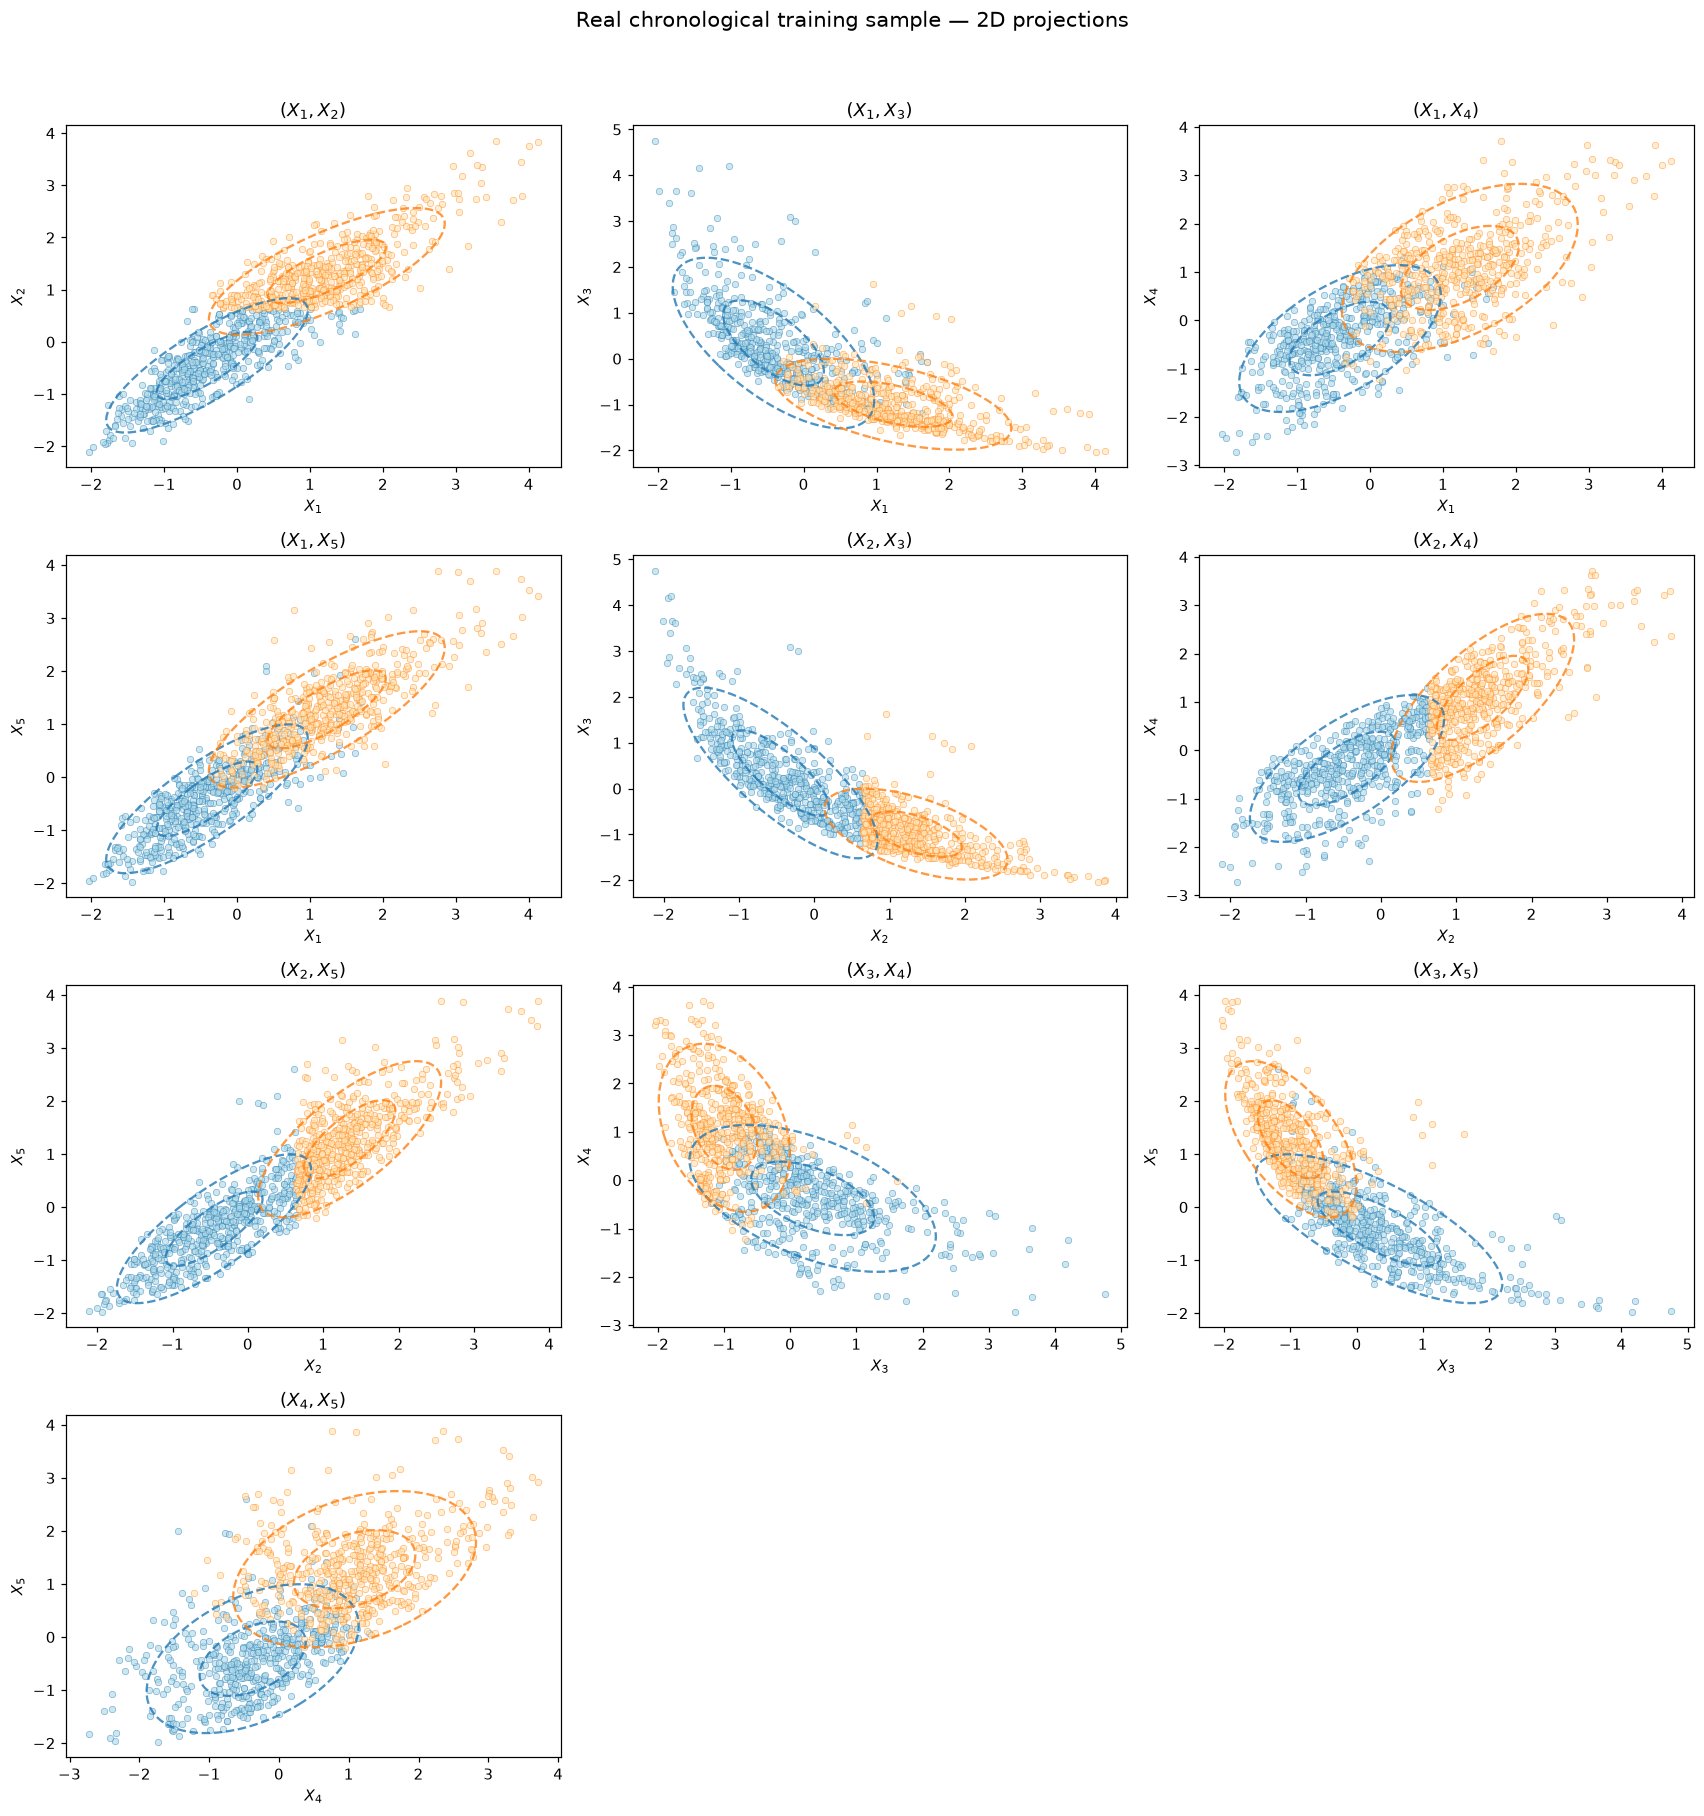
\includegraphics[width=\textwidth,height=0.85\textheight,keepaspectratio]{figures/geometry/air_quality/viz_2d_real_full_000005.png}
  \sourcebelow{relatório publicado do cenário Air Quality 000005 do \CoInfoSim}
\end{figure}

\begin{figure}[H]
  \centering
  \caption{Matriz completa de projeções --- UCI Air Quality, Gaussiana única}
  \label{fig:geom-air-full-gaussian}
  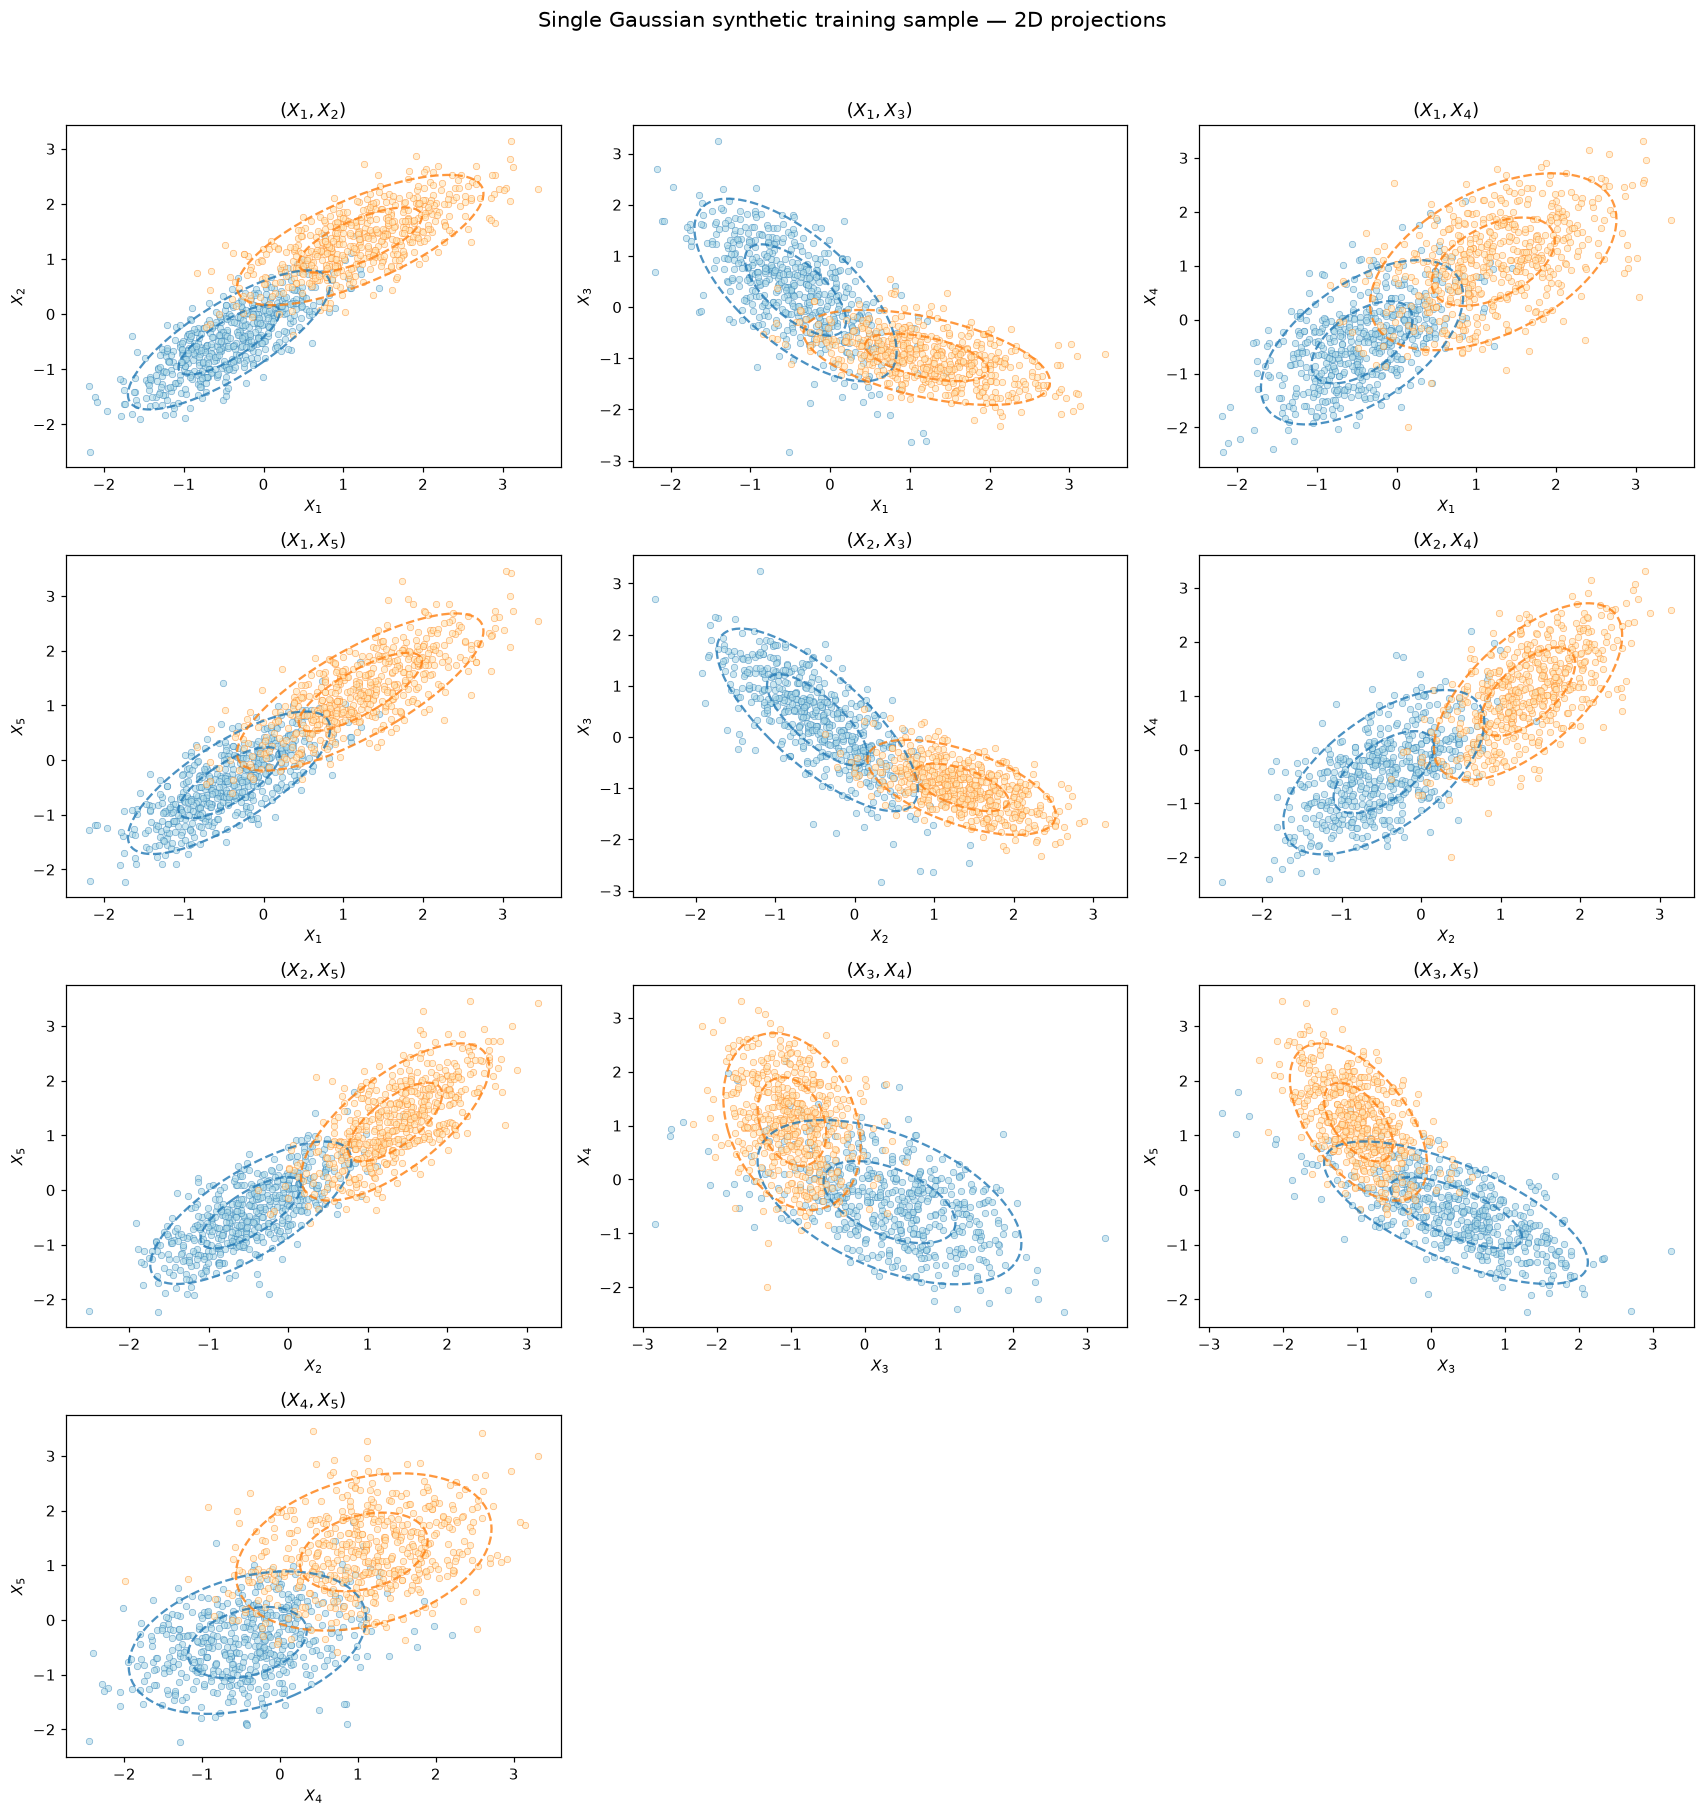
\includegraphics[width=\textwidth,height=0.85\textheight,keepaspectratio]{figures/geometry/air_quality/viz_2d_gaussian_full_000005.png}
  \sourcebelow{relatório publicado do cenário Air Quality 000005 do \CoInfoSim}
\end{figure}

\begin{figure}[H]
  \centering
  \caption{Matriz completa de projeções --- UCI Air Quality, GMM}
  \label{fig:geom-air-full-gmm}
  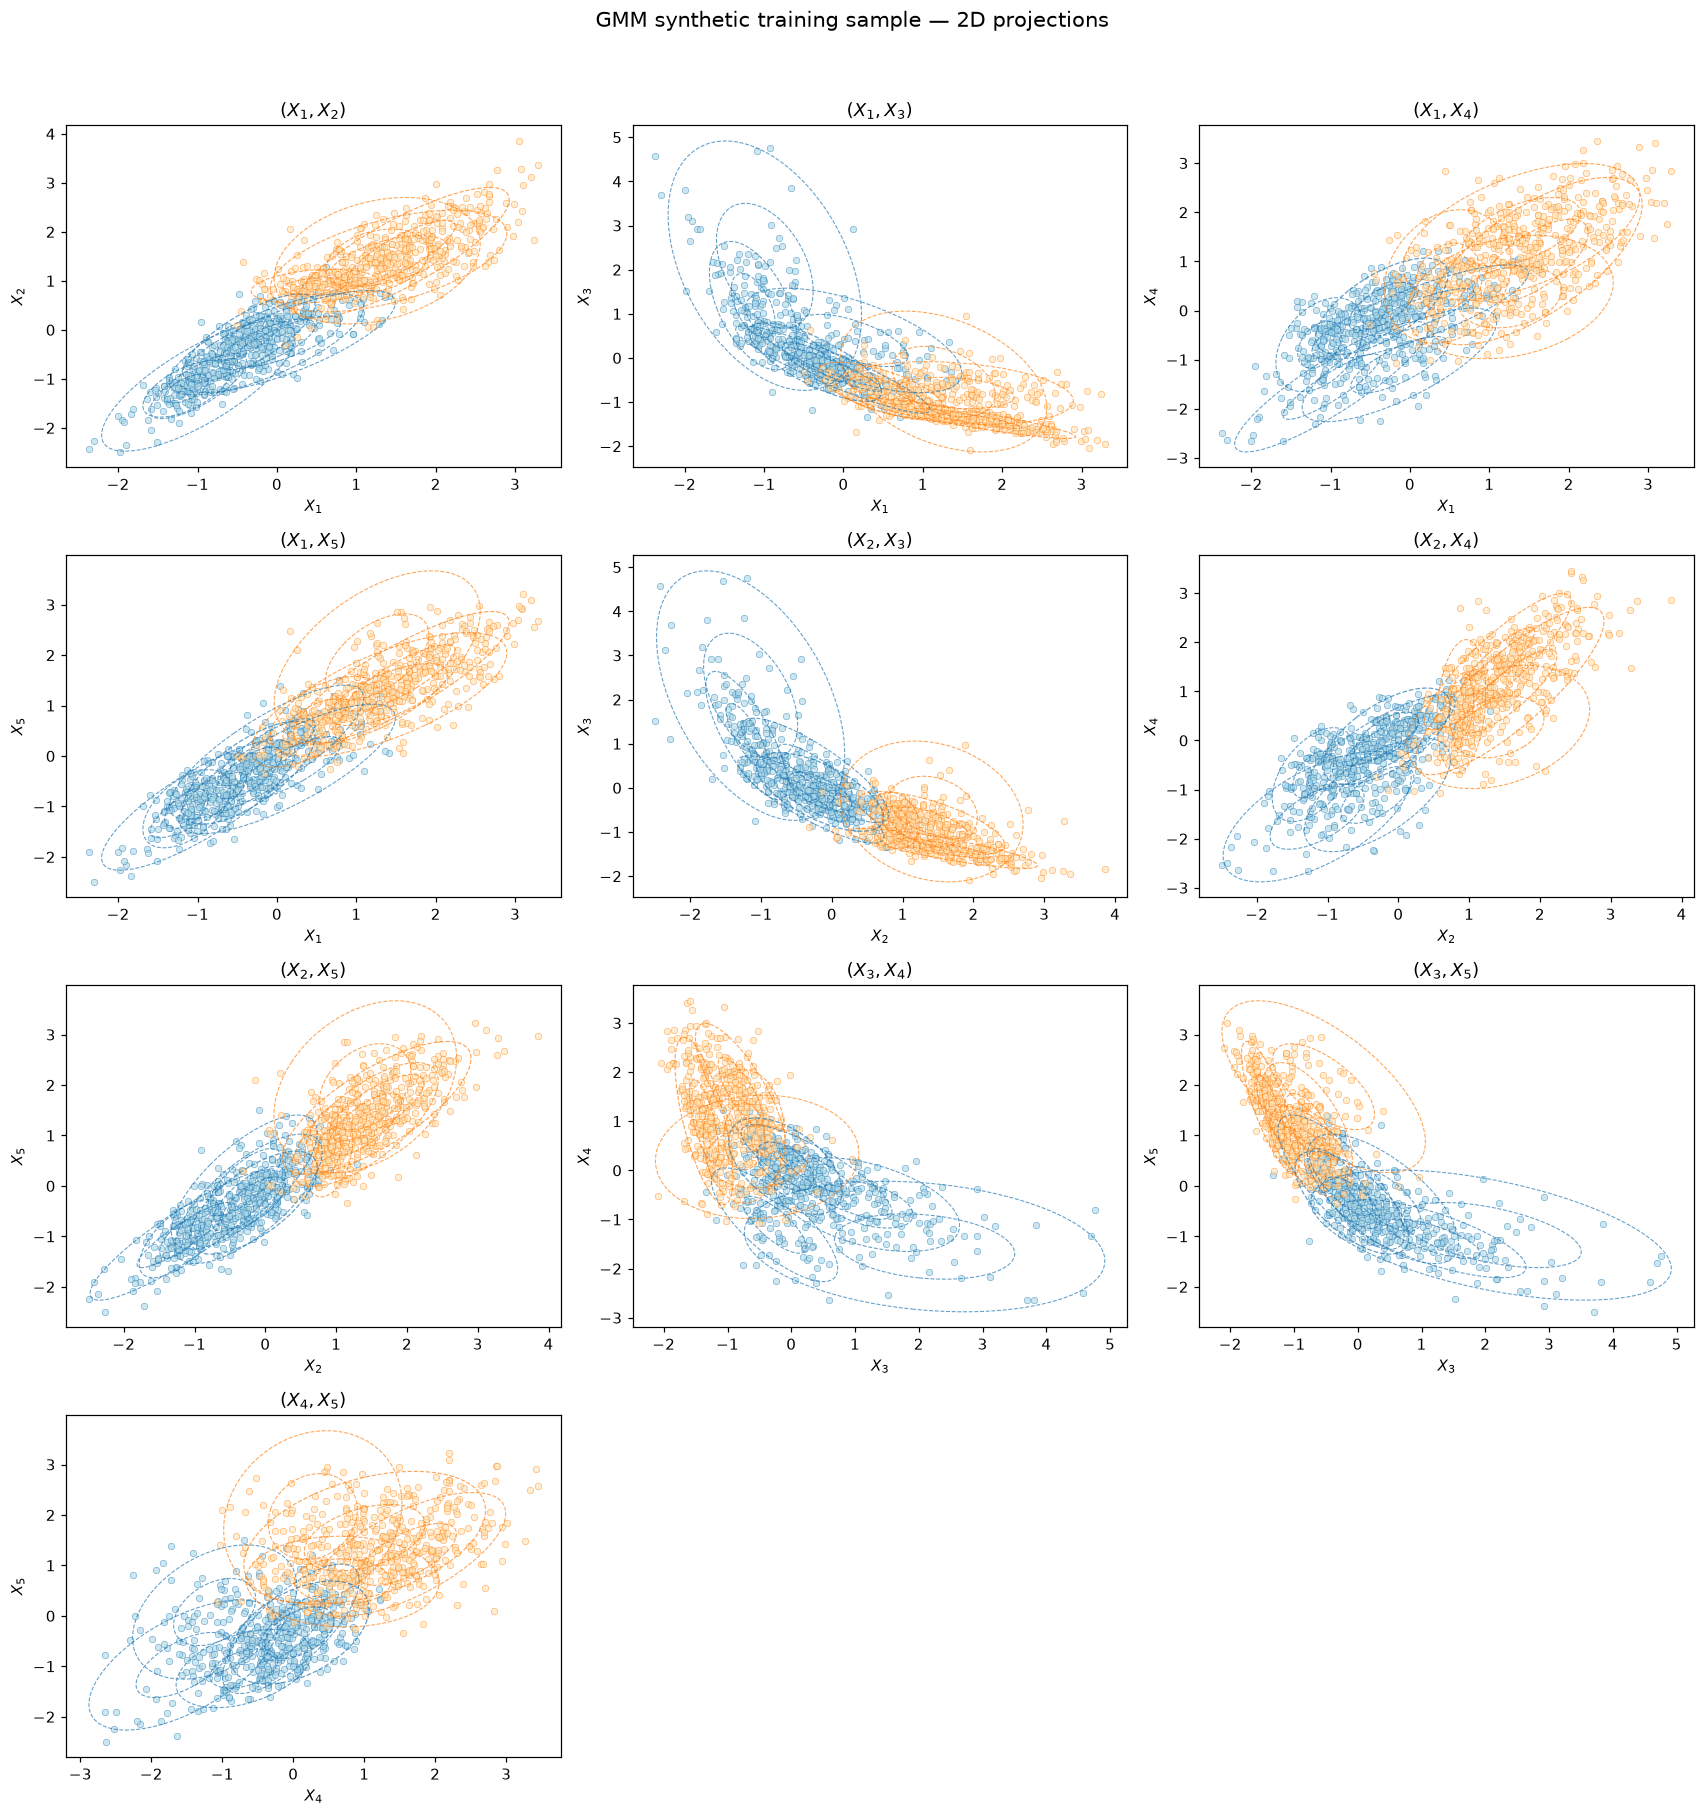
\includegraphics[width=\textwidth,height=0.85\textheight,keepaspectratio]{figures/geometry/air_quality/viz_2d_gmm_full_000005.png}
  \sourcebelow{relatório publicado do cenário Air Quality 000005 do \CoInfoSim}
\end{figure}

\begin{figure}[H]
  \centering
  \caption{Matriz completa de projeções --- SUPPORT2, dados reais}
  \label{fig:geom-support2-full-real}
  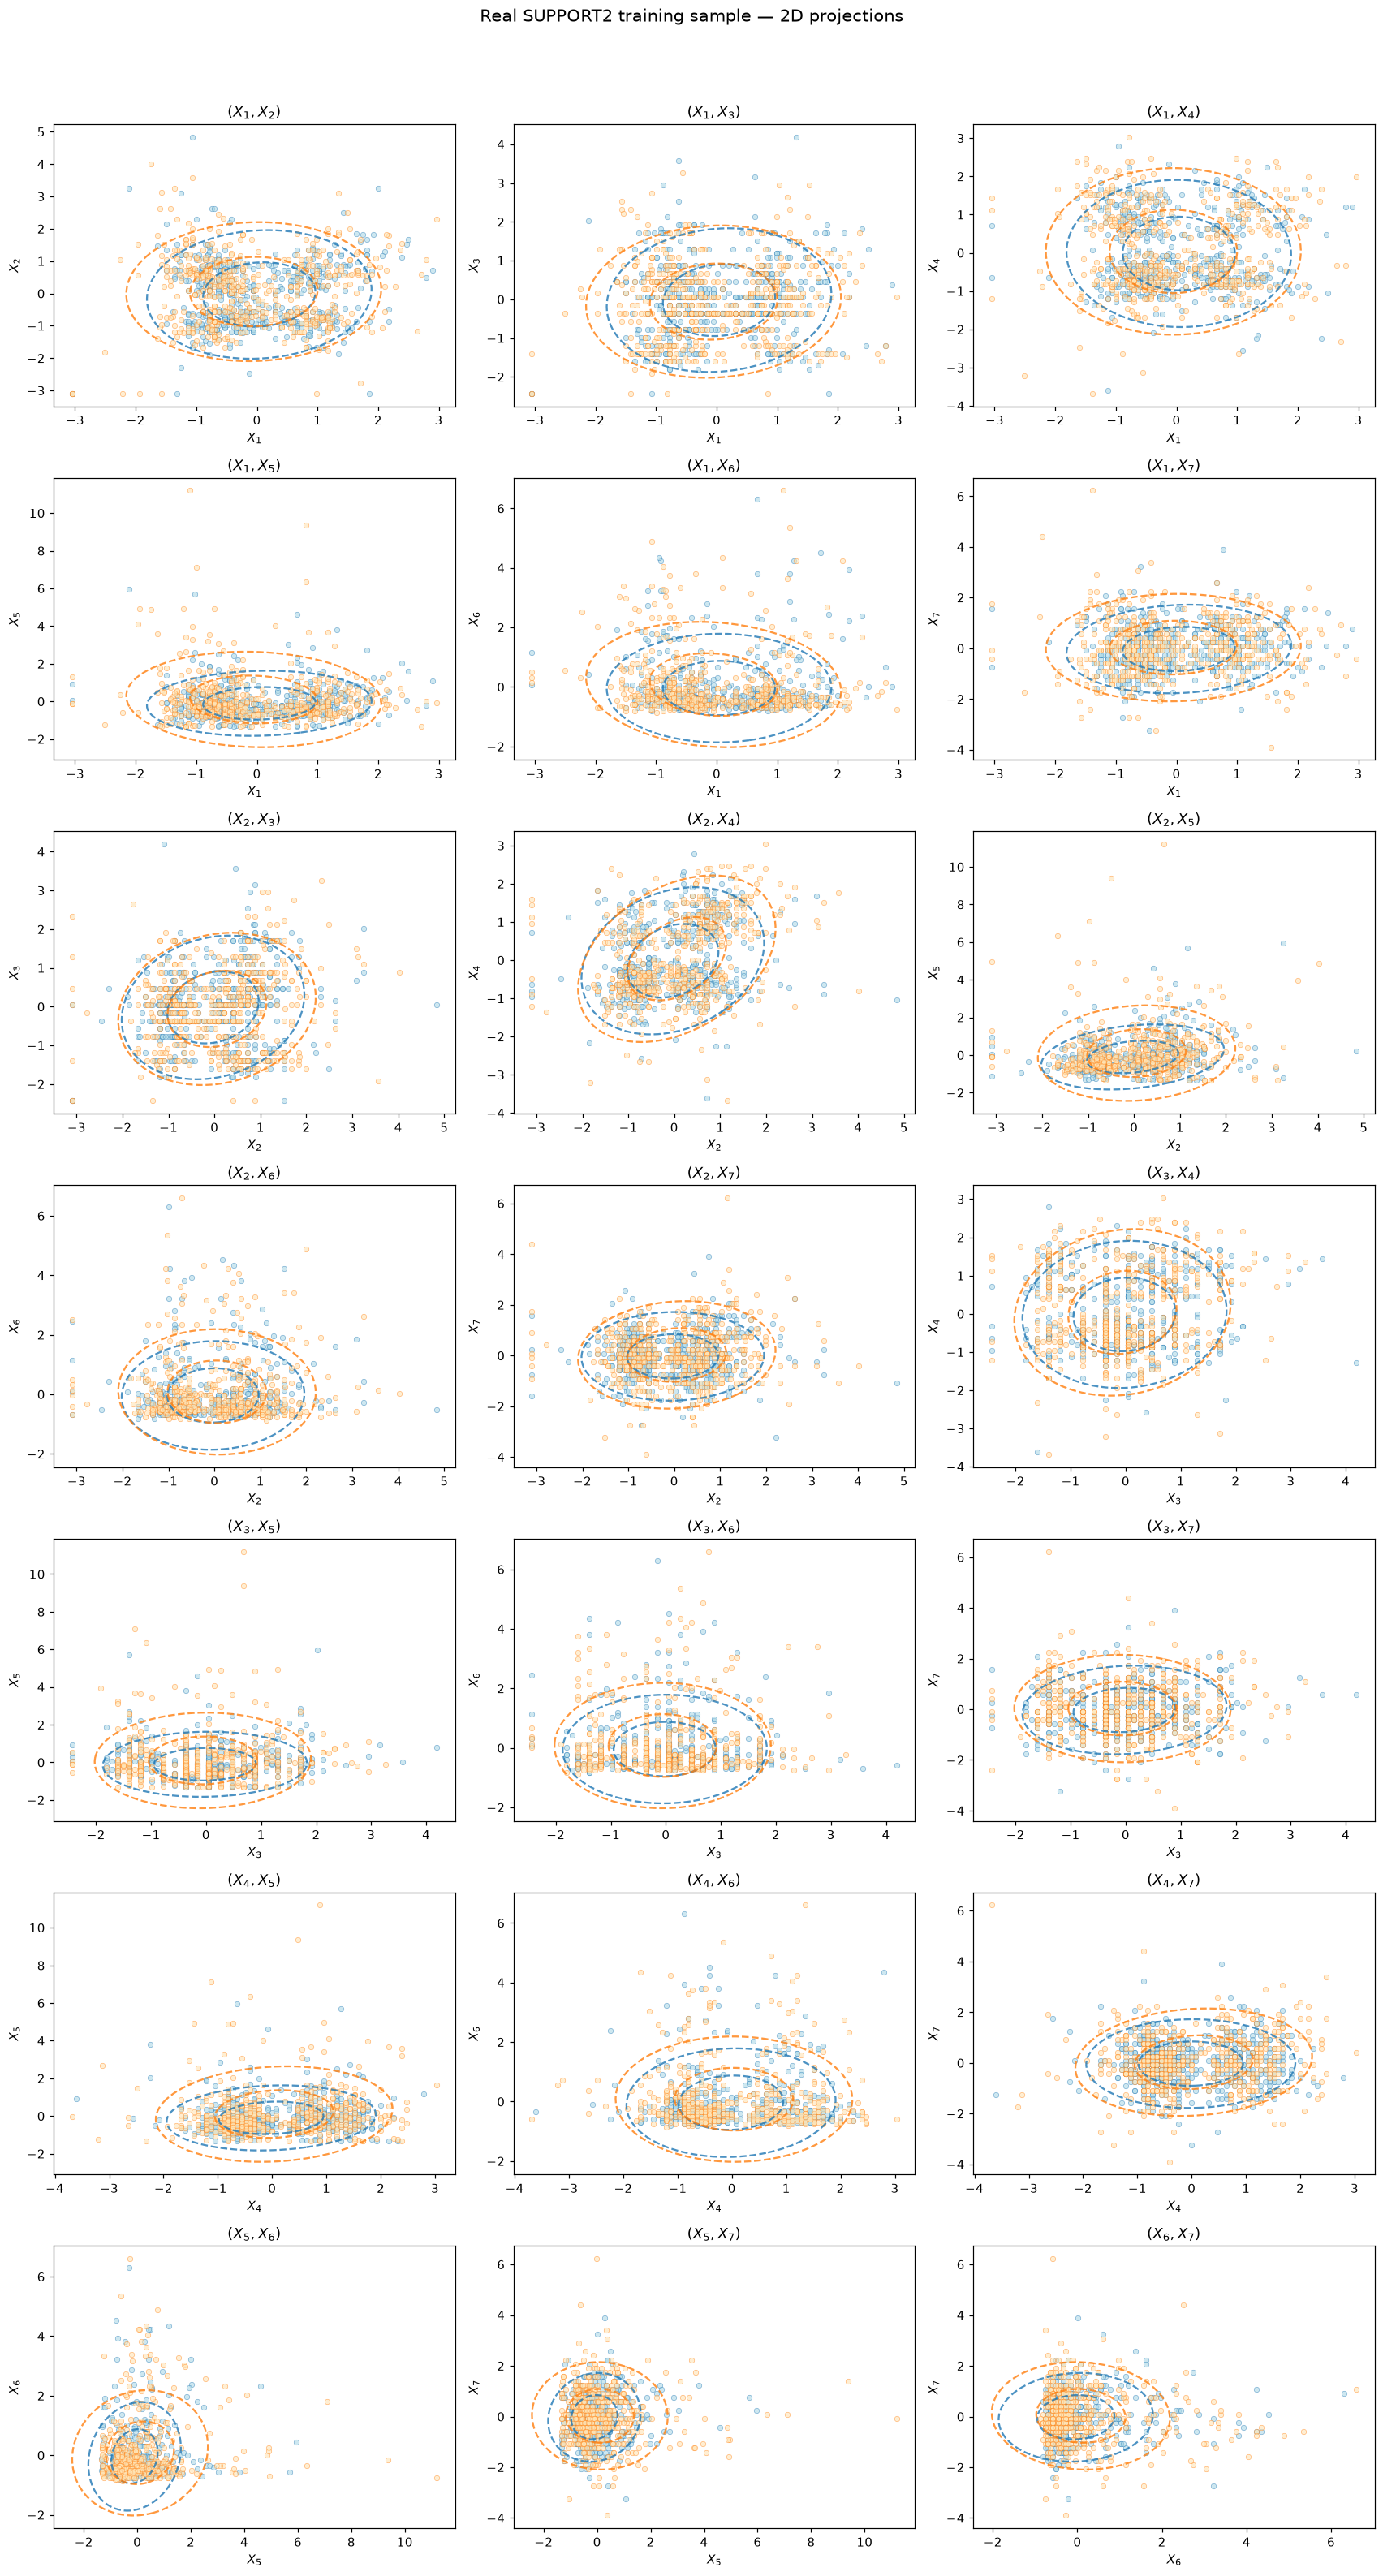
\includegraphics[width=\textwidth,height=0.85\textheight,keepaspectratio]{figures/geometry/support2/viz_2d_real_full_000008.png}
  \sourcebelow{relatório publicado do cenário SUPPORT2 000008 do \CoInfoSim}
\end{figure}

\begin{figure}[H]
  \centering
  \caption{Matriz completa de projeções --- SUPPORT2, Gaussiana única}
  \label{fig:geom-support2-full-gaussian}
  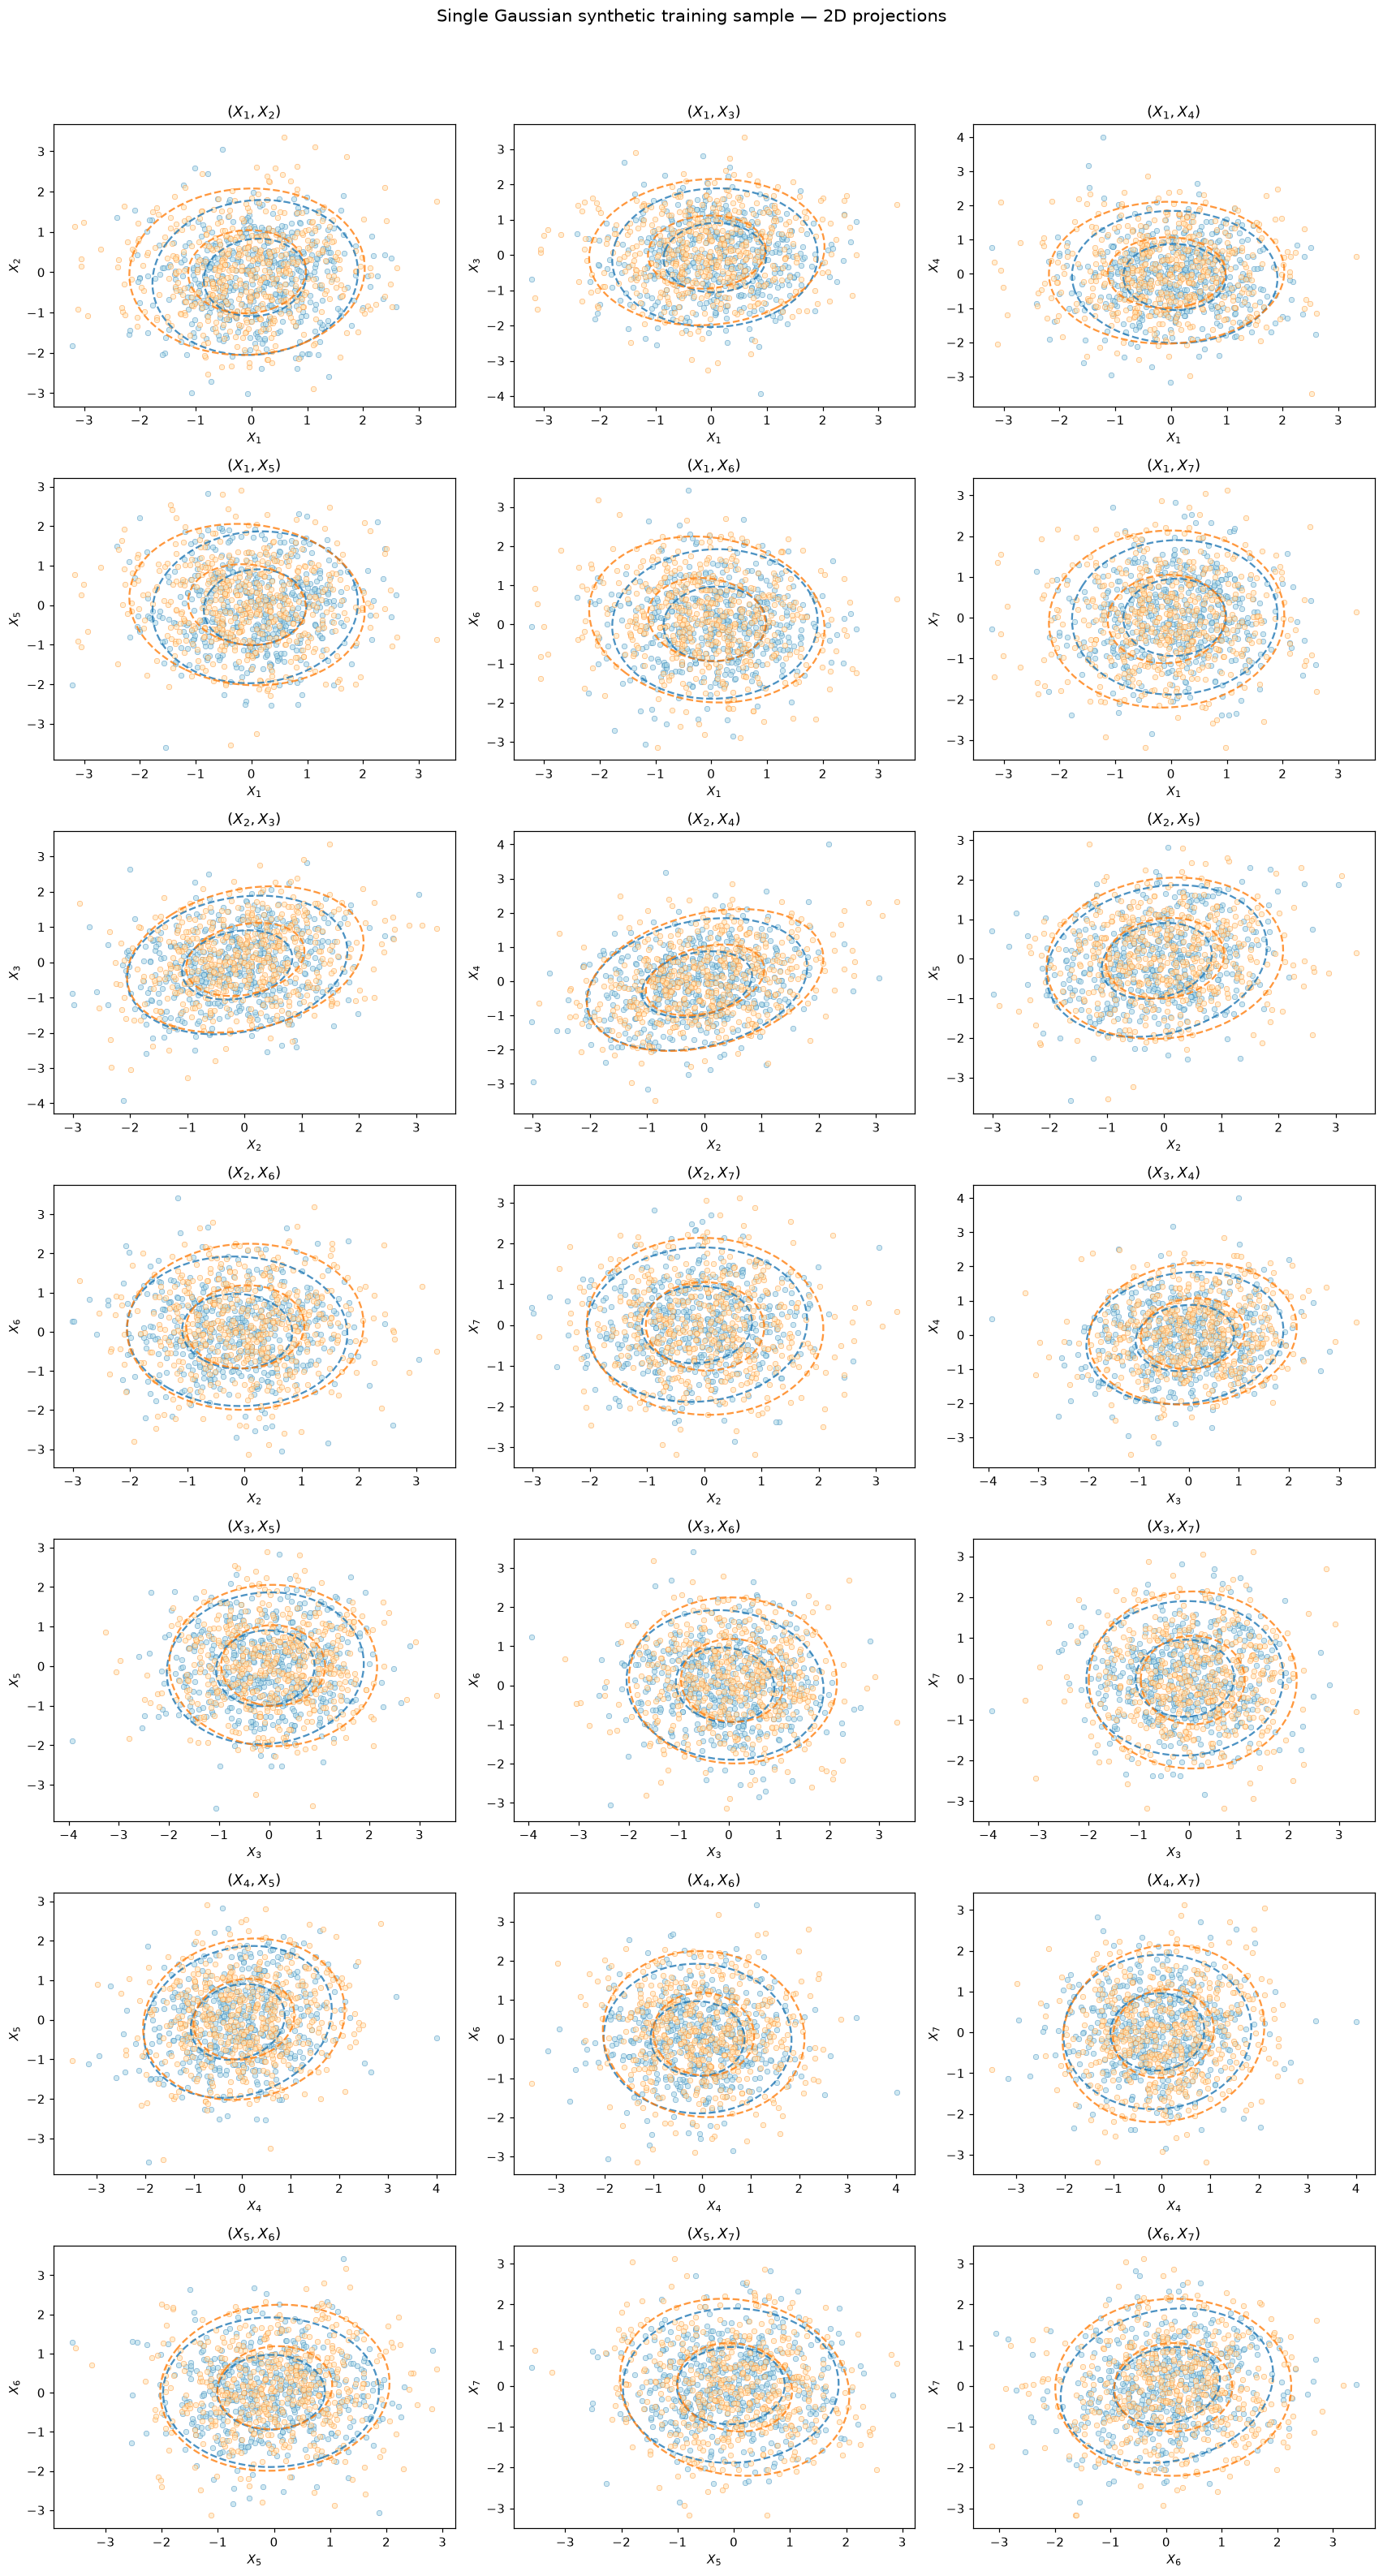
\includegraphics[width=\textwidth,height=0.85\textheight,keepaspectratio]{figures/geometry/support2/viz_2d_gaussian_full_000008.png}
  \sourcebelow{relatório publicado do cenário SUPPORT2 000008 do \CoInfoSim}
\end{figure}

\begin{figure}[H]
  \centering
  \caption{Matriz completa de projeções --- SUPPORT2, GMM}
  \label{fig:geom-support2-full-gmm}
  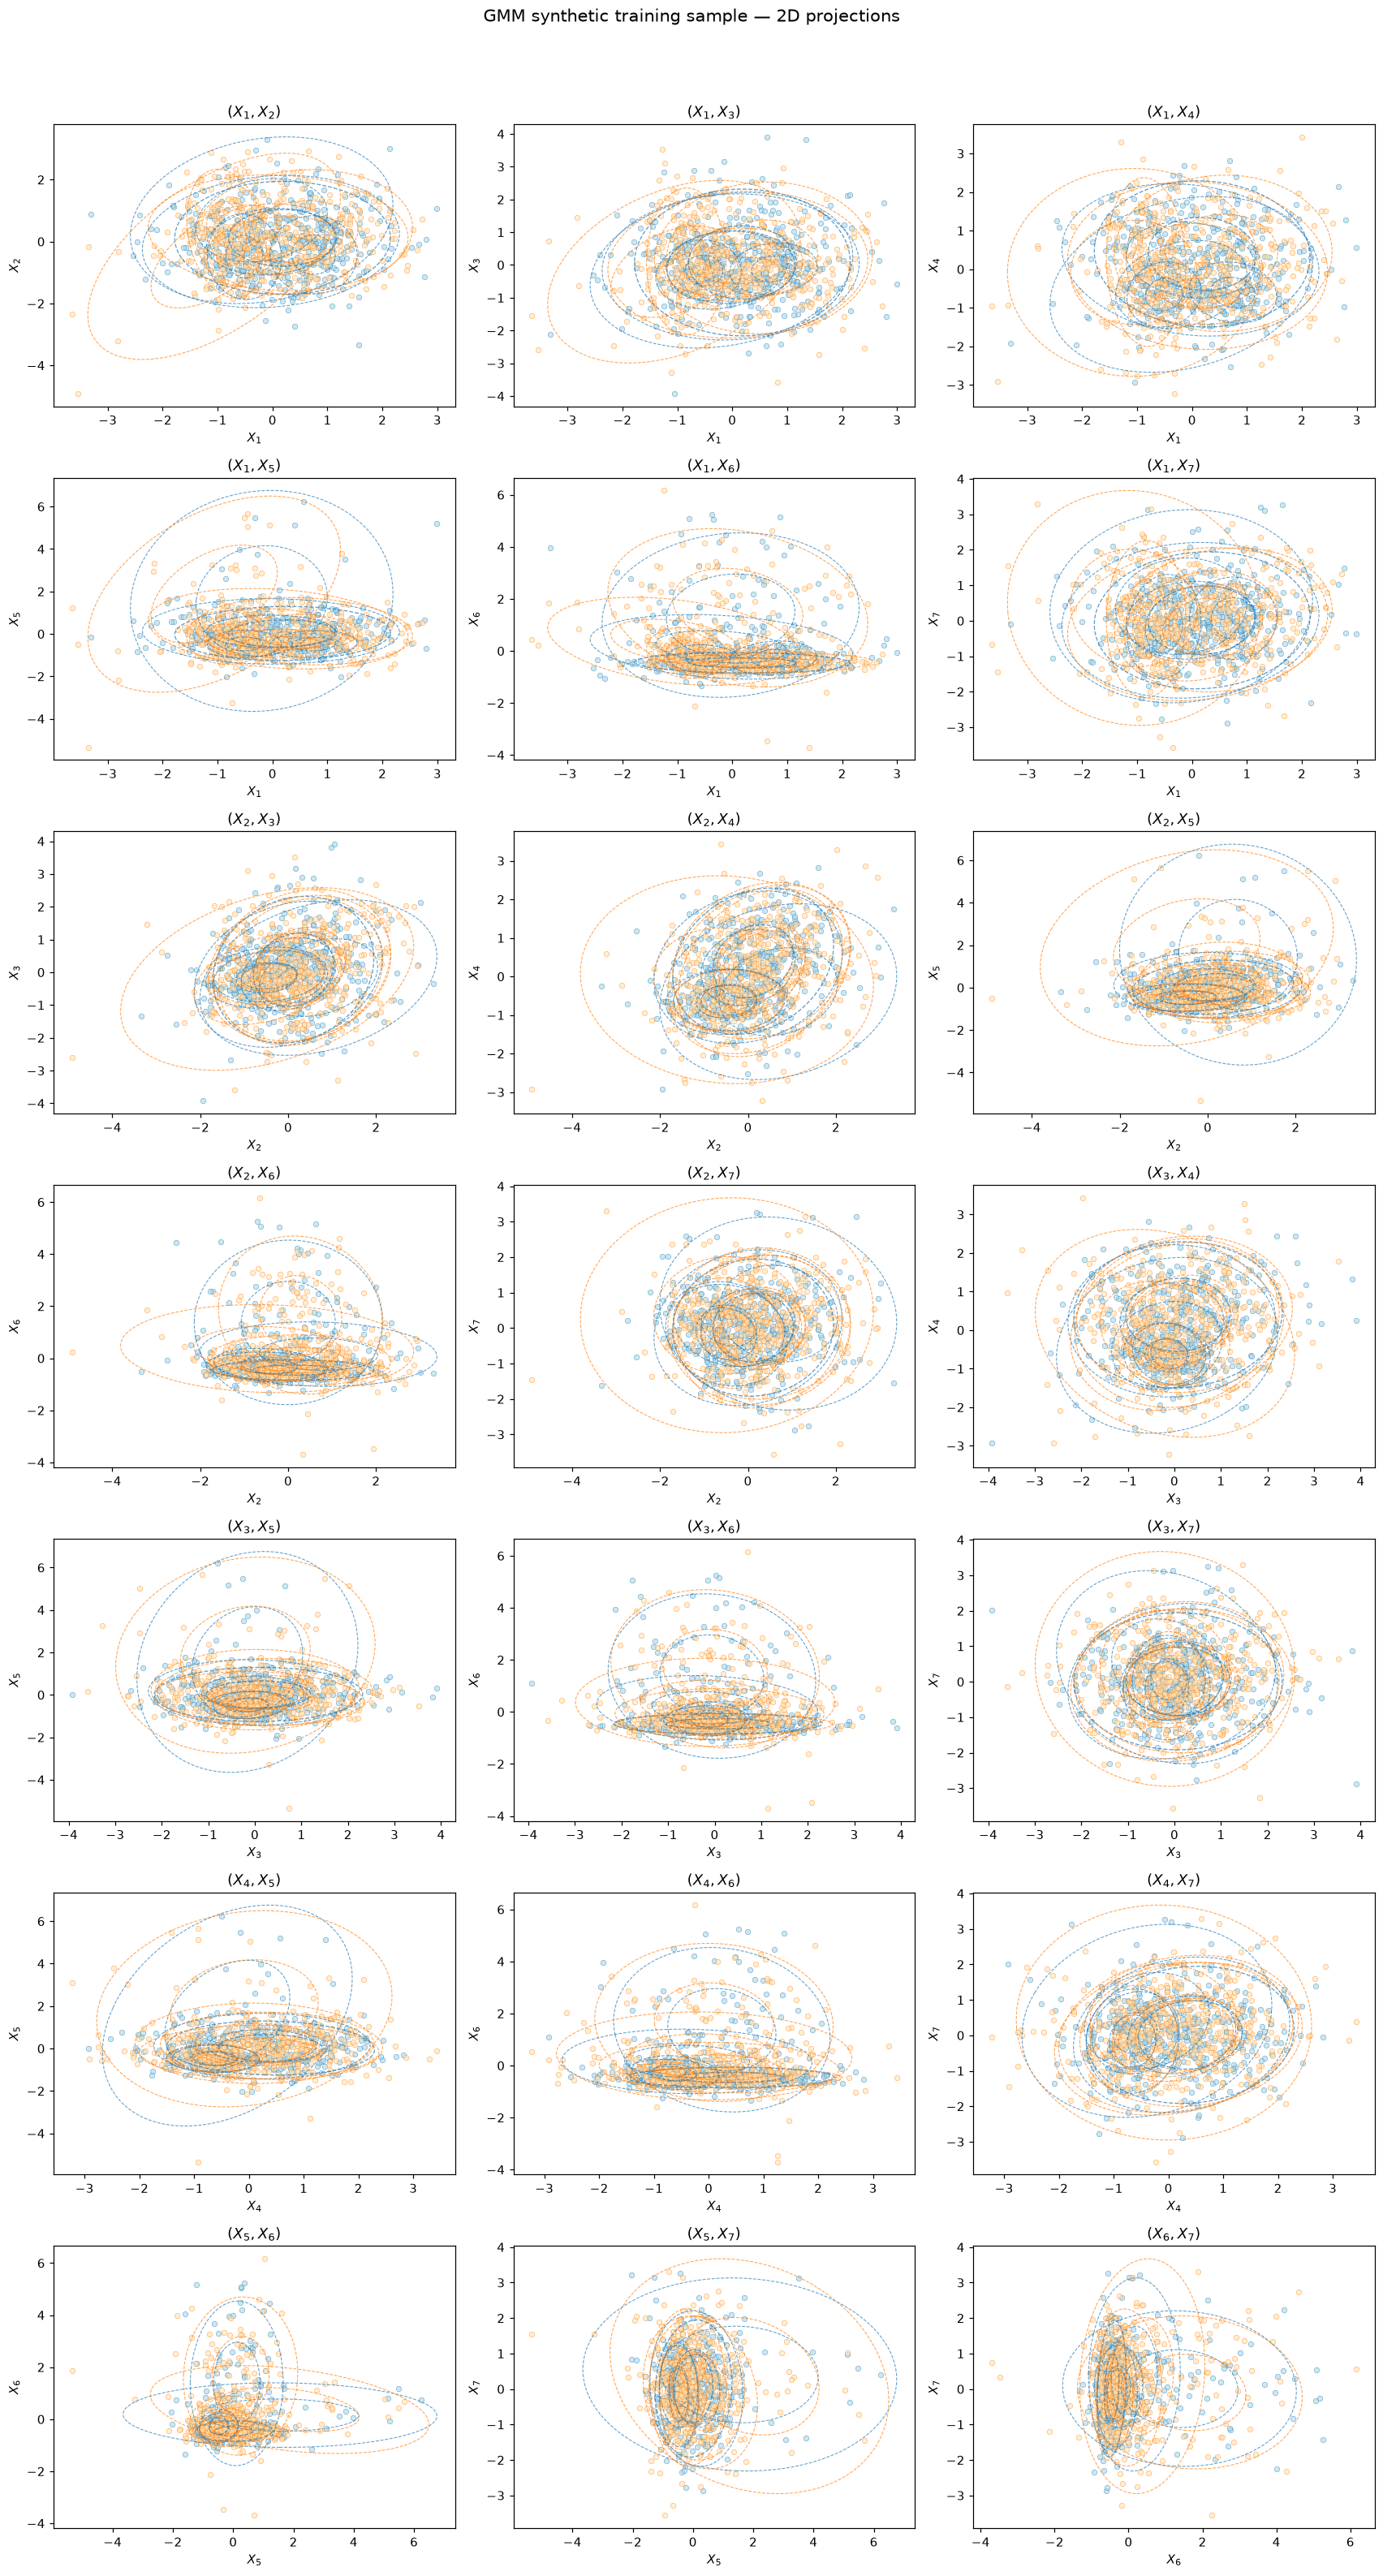
\includegraphics[width=\textwidth,height=0.85\textheight,keepaspectratio]{figures/geometry/support2/viz_2d_gmm_full_000008.png}
  \sourcebelow{relatório publicado do cenário SUPPORT2 000008 do \CoInfoSim}
\end{figure}

\section{Política de uso do material suplementar}

Os relatórios online listados na Seção~\ref{ap:resultados-cenarios} são a fonte exaustiva dos resultados desta revisão, incluindo as matrizes $\Wmat$/$\Rmat$ completas de cada cenário. O PDF não reproduz todas as matrizes e curvas porque isso prejudicaria a leitura e duplicaria centenas de visualizações; ele apresenta uma seleção orientada pelas hipóteses científicas, com os quatro indicadores tabulados por completo e ilustrados por figuras de evolução por $n$ (Capítulo~5). A rastreabilidade é preservada por meio dos IDs imutáveis de cenário e simulação, nomes de arquivos, parâmetros registrados e resultados JSON persistidos no ambiente auditado. Todos os resultados apresentados neste relatório, em texto, tabelas e figuras, são de execuções \textit{full} ou \textit{full-scale}; nenhum resultado de execução \textit{smoke} é reportado como evidência --- o modo \textit{smoke} do \CoInfoSim{} é usado apenas para testes e validação computacional do próprio código (Apêndice~B), nunca como fonte de resultados científicos.

Os gráficos vetoriais de $\rankrho$/$\AW$ reconstruídos a partir de tabelas finais publicadas anteriormente para Occupancy e Air Quality (identificados individualmente em \texttt{figures/FIGURE\_SOURCES.md} e nas fontes de cada figura no corpo do texto) foram incorporados sem recortes que alterassem eixos, ordem dos subconjuntos, escala ou legenda; os valores de $\rankrho$/$\AW$ que ilustram foram confirmados computacionalmente nesta revisão a partir dos resultados brutos regenerados, dentro da precisão de transcrição das versões anteriores (Seção~\ref{sec:resultados-guia}). As matrizes $\Wmat$/$\Rmat$ do SUPPORT2 (Figura~\ref{fig:wr-matrices-support2-appendix}, Apêndice~D) e as figuras de evolução dos quatro indicadores por $n$ (Capítulo~5) foram geradas diretamente pelas funções vigentes de \texttt{coinfosim.reports.predictive\_profile\_visualization} sobre os resultados brutos regenerados dos quatro cenários de escala completa. Os valores de $\AR$, $\DR$ e $\SR$ apresentados em todas as tabelas do Capítulo~5 foram computados diretamente pelo código atual sobre resultados brutos por replicação, sem reconstrução a partir de nenhuma tabela ou figura publicada anteriormente.
